\spacing{1.25}
En este capítulo se presentan los resultados de las simulaciones de chubascos iniciados por rayos cósmicos de energías entre $10^{17.256}$ y $10^{19.626}$ eV, considerando la composición mixta de rayos cósmicos primarios basada en datos del Observatorio Pierre Auger. Se muestran los resultados de dos observables: la profundidad del máximo y su desviación estándar. Se comparan tres modelos de interacción hadrónica con los que se realizaron las simulaciones, además de comparar los resultados obtenidos con los respectivos datos observacionales. \\

Se simularon 2400 chubascos en el rango de energías mencionado, en la ubicación de Malargue -donde se encuentra una de las estaciones del Pierre Auger-, con ángulo zenital entre 0$^{o}$ y 70$^{o}$ y ángulo azimutal distribuido isotrópicamente entre 0$^{o}$ y 360$^{o}$. La simulaciones se realizaron con tres modelos de interacción hadrónica: Sibyll 2.3c, EPOS-LHC y QGSJETII-04, tomando en cuenta la composición primaria mixta (una combinación de protones, núcleos de helio, nitrógeno y hierro) propuesta por la colaboración Pierre Auger en \cite{PAOcomposition}, mostrada en la Fig. \ref{fig:composition}.

\begin{center}
\begin{figure}[h]
\centering
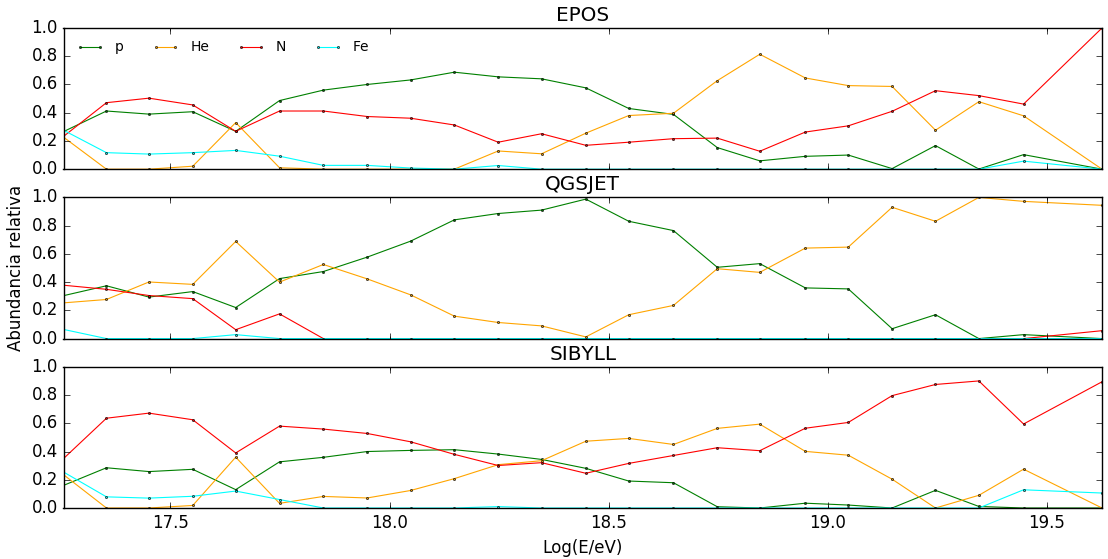
\includegraphics[height=0.3\textheight]{Figuras/composition} 
\caption{Composición en función de la energía, resultado de un ajuste con los datos del Observatorio Pierre Auger.}
\label{fig:composition}
\end{figure}	
\end{center}

\section{Profundidad del máximo $X_{max}$}
\subsection{Comparación de predicciones de los modelos hadrónicos}
Se calculó el promedio de la profundidad del máximo de 100 eventos para cada energía realizando el correspondiente ajuste mediante el algoritmo de mínimos cuadrados no lineal Levenberg-Marquardt. En la gráfica de la Fig. \ref{fig:Xmodelos} se muestran los resultados de $X_{max}$ para los tres modelos hadrónicos.\\

\begin{figure}[h]
\centering
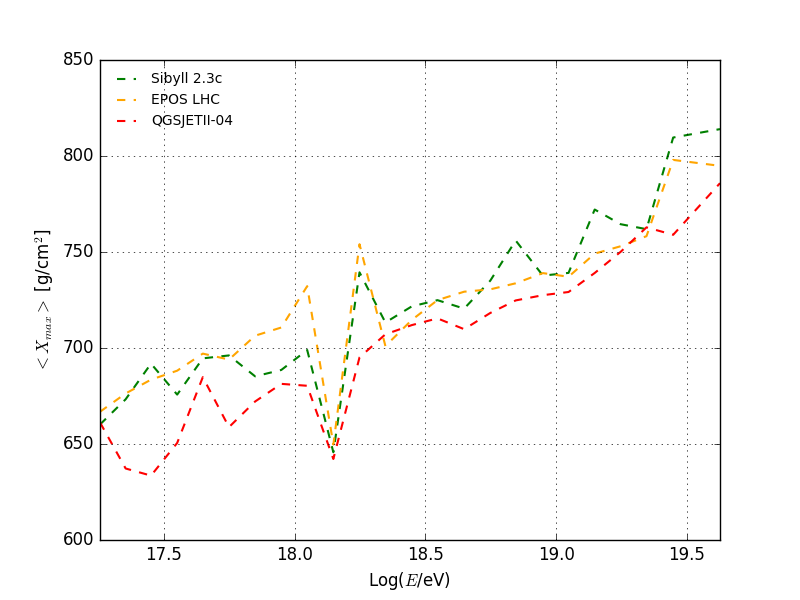
\includegraphics[width=0.7\textwidth]{Figuras/Xmax_modelos} 
\caption{$X_{max}$ promedio resultante de las simulaciones con los modelos hadrónicos Sibyll 2.3c, EPOS-LHC y QGSJETII-04}
\label{fig:Xmodelos}
\end{figure}	

Se observa que en general los tres modelos muestran la misma tendencia de crecimiento de $X_{max}$ con la energía, sin embargo el modelo QGSJET es el que más difiere de los otros dos modelos, prediciendo el máximo a una menor profundidad, con una diferencia promedio de aproximadamente 3\%, mientras que Sibyll y EPOS difieren entre ellos un 1.5\% en promedio.

\begin{table}[h]
\centering
\caption{Diferencias porcentuales entre los resultados de $X_{max}$ de los distintos modelos de interacción hadrónica.}
\begin{tabular}{l|ccc}
\hline
              & \multicolumn{1}{l}{Dif. media (\%)} & \multicolumn{1}{l}{Mín. (\%)} & \multicolumn{1}{l}{Máx. (\%)} \\ \hline
Sibyll/QGSJET & 2.914                               & 0.123                         & 9.207                         \\ \hline
EPOS/QGSJET   & 3.085                               & 0.379                         & 8.484                         \\ \hline
Sibyll/EPOS   & 1.473                               & 0.003                         & 4.544  						  \\ \hline 
\end{tabular}
\label{modeldif} 
\end{table}

\subsection{Comparación con datos observacionales}
En la figura Fig. \ref{fig:Xobs} se muestran tanto los resultados de las simulaciones como los datos obtenidos por el Observatorio Pierre Auger. Los modelos Sibyll y EPOS muestran excelente concordancia con las observaciones en las energías más bajas del rango considerado, luego de $E\approx 10^{18.248}$ eV los datos simulados son en general menores que los experimentales. Por otro lado, QGSJET tiende a subestimar la profundidad del máximo de los chubascos en todo el rango de energías.\\

\begin{figure}[h]
\centering
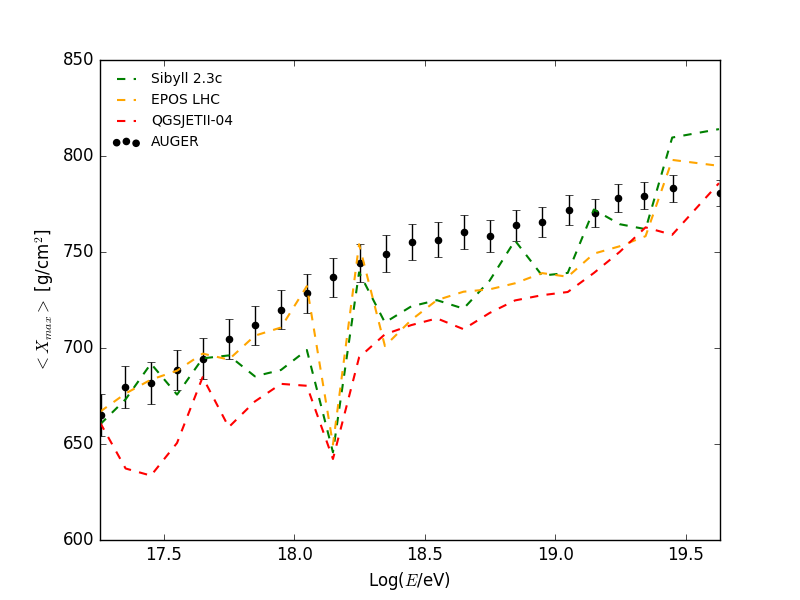
\includegraphics[width=0.7\textwidth]{Figuras/Xmax_modelos_obs} 
\caption{$X_{max}$ promedio resultante de las simulaciones con los modelos hadrónicos Sibyll 2.3c, EPOS-LHC y QGSJETII-04 junto con los datos tomados por el Observatorio Pierre Auger. Las barras representan el error sisteático de las medidas.}
\label{fig:Xobs}
\end{figure}	

Para toda la ventana de energías, el modelo EPOS es el que mejor reproduce los datos del Pierre Auger, con un error relativo de 2.8\% en promedio, le sigue Sibyll con 3.1\% y por último está QGSJET con 5.1\% de error relativo.\\

\begin{table}[h]
\centering
\caption{Error porcentual de los resultados de $X_{max}$ de las simulaciones relativo a los datos observacionales.}
\begin{tabular}{l|ccc}
\hline
Modelo & Err. relativo (\%) & Mín. (\%) & Máx. (\%) \\ \hline
Sibyll & 3.080              & 0.023     & 12.364    \\ \hline
EPOS   & 2.778              & 0.050     & 11.820    \\ \hline
QGSJET & 5.092              & 0.589     & 12.840    \\ \hline
\end{tabular}
\end{table}

La subestimación de $X_{max}$ en las simulaciones puede sugerir que en las mayores energías, los chubascos se producen por rayos cósmicos de composición más ligera que la que se ha considerado. Sin embargo, como evidencian las discrepancias entre los modelos, la reproducción de los datos observacionales es altamente dependiente del modelo hadrónico utilizado y de sus características particulares.


\section{Desviación estándar del máximo $\sigma X_{max}$}
\subsection{Comparación de predicciones de los modelos hadrónicos}
Las fluctuaciones de la profundidad del máximo de un chubasco a otro con la misma energía es una magnitud que también es sensible a la composición primaria. En la Fig. \ref{fig:Smodelos} se muestran los resultados de las simulaciones para esta observable. \\

\begin{figure}[h]
\centering
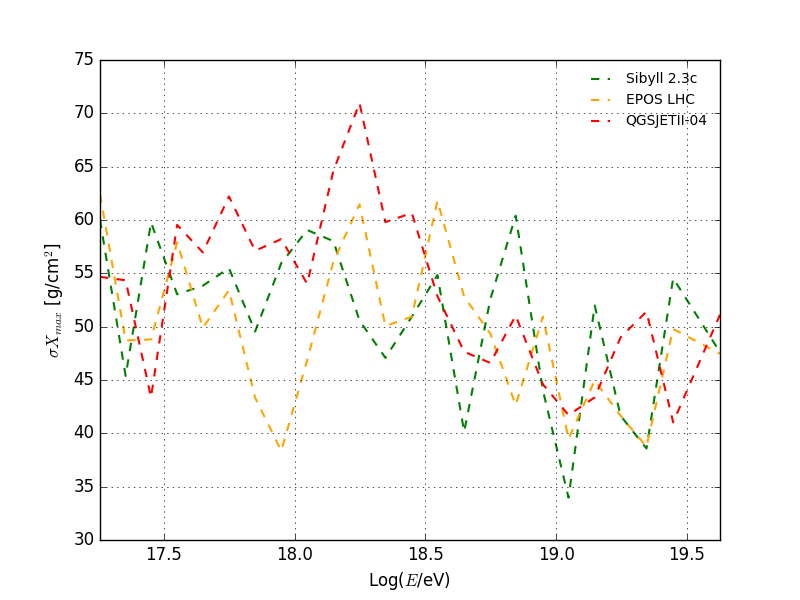
\includegraphics[width=0.7\textwidth]{Figuras/StddvXmax_modelos} 
\caption{Fluctuaciones en el valor de profundidad del máximo $\sigma X_{max}$ resultante de las simulaciones con los modelos hadrónicos Sibyll 2.3c, EPOS-LHC y QGSJETII-04.}
\label{fig:Smodelos}
\end{figure}	

En el caso de $\sigma X_{max}$ se observa que los tres modelos hadrónicos difieren de manera notable entre sí. Las diferencias se encuentran alrededor de 15\% en casi todo el rango de interés, a pesar de coincidir en puntos aislados. No se observa una tendencia clara de los datos simulados.

\begin{table}[h]
\centering
\caption{Diferencias porcentuales entre los resultados de $\sigma X_{max}$ de los distintos modelos de interacción hadrónica.}
\begin{tabular}{l|ccc}
\hline
              & Dif. media (\%) & Mín. (\%) & Máx. (\%) \\ \hline
Sibyll/QGSJET & 15.168          & 1.256     & 37.782    \\ \hline
EPOS/QGSJET   & 14.089          & 2.721     & 34.101    \\ \hline
Sibyll/EPOS   & 12.651          & 0.000     & 45.881    \\ \hline
\end{tabular}
\end{table}

\subsection{Comparación con datos observacionales}
En la Fig. \ref{fig:Sobs} se muestran los datos experimentales $\sigma X_{max}$ junto con los resultados de las simulaciones. Es evidente que el modelo que mejor reproduce la tendencia de los datos es QGSJET, principalmente en la parte central del rango desde $\sim 10^{17.551}$ hasta $\sim 10^{18.845}$. En las menores energías QGSJET subestima las fluctuaciones, mientras que en las mayores las sobreestima. Las predicciones de EPOS y Sibyll están en general más bajas que los datos, con excepción de las mayores energías donde los tres modelos están por encima de los datos de l Pierre Auger.\\

\begin{figure}[h]
\centering
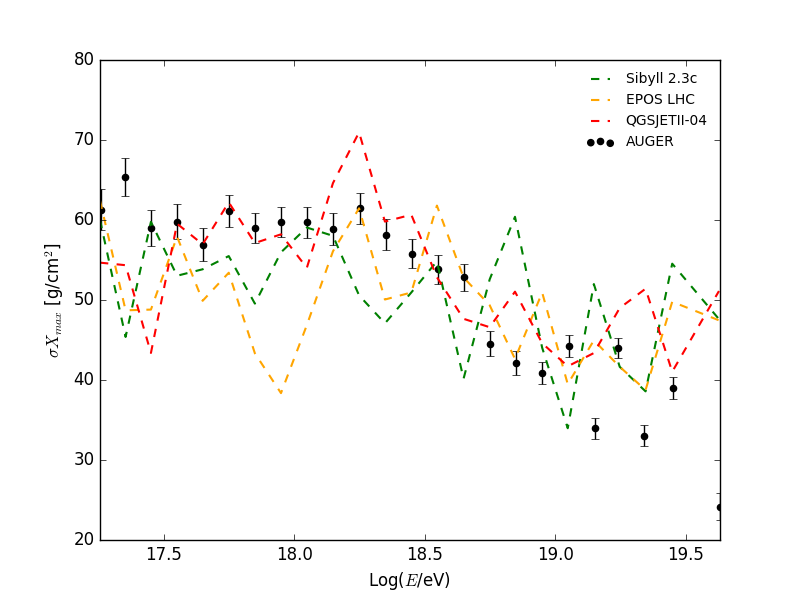
\includegraphics[width=0.7\textwidth]{Figuras/StddvXmax_modelos_obs} 
\caption{Fluctuaciones en el valor de profundidad del máximo $\sigma X_{max}$ resultantes de las simulaciones con los modelos hadrónicos Sibyll 2.3c, EPOS-LHC y QGSJETII-04 junto con los datos tomados por el Observatorio Pierre Auger. Las barras representan el error sisteático de las medidas.}
\label{fig:Sobs}
\end{figure}	

Ninguno de los tres modelos hadrónicos utilizados reproduce fielmente la desviación estándar de la profundidad del máximo, con errores del 18\% en promedio pero que llegan a ser de más del 30\% en varios puntos. Esto puede deberse principalmente a la cantidad de chubascos simulados con una misma energía, que está bastante por debajo de la cantidad de eventos observados a bajas energías, y por el contrario está por encima de los eventos observados a más altas energías. De manera que la cantidad de simulaciones realizadas puede estar afectando las fluctuaciones de chubasco a chubasco, no obstante estas diferencias con los datos observacionales no parecen indicar un cambio claro en la composición primaria.

\begin{table}[h]
\centering
\caption{Error porcentual de los resultados de $\sigma X_{max}$ de las simulaciones relativo a los datos observacionales.}
\begin{tabular}{l|ccc}
\hline
Modelo & Err. relativo (\%) & Mín. (\%) & Máx. (\%) \\ \hline
Sibyll & 19.192             & 1.072     & 97.143    \\ \hline
EPOS   & 17.722             & 0.016     & 96.522    \\ \hline
QGSJET & 15.509             & 0.053     & 111.677   \\ \hline
\end{tabular}
\end{table}

\singlespacing